\section{Definición de componentes comunes}
\label{sub:componentes_comunes}

En esta seccíón se pretende ubicar a los bloques que hacen a la base del
lenguaje, cuestiones que se utilizan como herramientas para definir otros
componentes mas complejos.

\subsection{letra}
\label{sub:letra}

Segun la notación BNF se tiene lo siguiente:

\begin{lstlisting} [basicstyle=\footnotesize\ttfamily]
	<letra> ::= a | b | c | d | e | f | g | h | i | j | k | l | m | n |
	o | p | q | r | s | t | u | v | w | x | y | z | A | B | C | D |
	E | F | G | H	| I | J | K | L | M | N | O | P | Q | R | S | T |
	U | V | W | X | Y | Z
\end{lstlisting}


y para un patrón para el motor de expresiones regulares se tiene lo
siguiente para las letras:

\begin{lstlisting}[basicstyle=\footnotesize\ttfamily]
Regex: /[a-zA-Z]/
\end{lstlisting}

\subsection{digito}
\label{sub:digito}
La notación para la gramática libre de contexto en formato BNF para los
\texttt{dígitos} es la siguiente:

\begin{lstlisting}[basicstyle=\footnotesize\ttfamily]
  <digito> ::= 0 | 1 | 2 | 3 | 4 | 5 | 6 | 7 | 8 | 9
\end{lstlisting}

En cuanto a la expresión regular para los mismos se define de la siguiente
manera:

\begin{lstlisting}[basicstyle=\footnotesize\ttfamily]
	Regex: /[0-9]/
\end{lstlisting}

\subsection{simbolo}
\label{sub:simbolo}
BNF para describir un simbolo dentro del lenguaje se expone a continuación:

\begin{lstlisting}[basicstyle=\footnotesize\ttfamily]
	<simbolo> ::= "|" | " " | "!" | "#" | "$" | "%" | "&" | "(" | ")"
	| "*" | "+"	| "," | "-" | "." | "/" | ":" | ";" | ">" | "=" | "<"
	| "?" | "@" | "[" | "\"	| "]" | "^" | "_" | "`" | "{" | "}" | "~"
\end{lstlisting}


\subsection{texto}
\label{sub:texto}
La definición de este elemento simplifica futuro manejo de cuestiones dentro de
la definición del lenguaje, el elemento \texttt{texto} es la aplicación
sucesiva de los elementos \texttt{letra}, \texttt{digito} y \texttt{simbolo}.

El BNF para el elemento se describe de la siguiente manera:

\begin{lstlisting}[basicstyle=\footnotesize\ttfamily]
  <texto> ::= <letra|digito|simbolo> <texto>
\end{lstlisting}

El autómata finito para este explica al relación de los tres elementos
mencionados:

\begin{figure}[H]
	\centering
	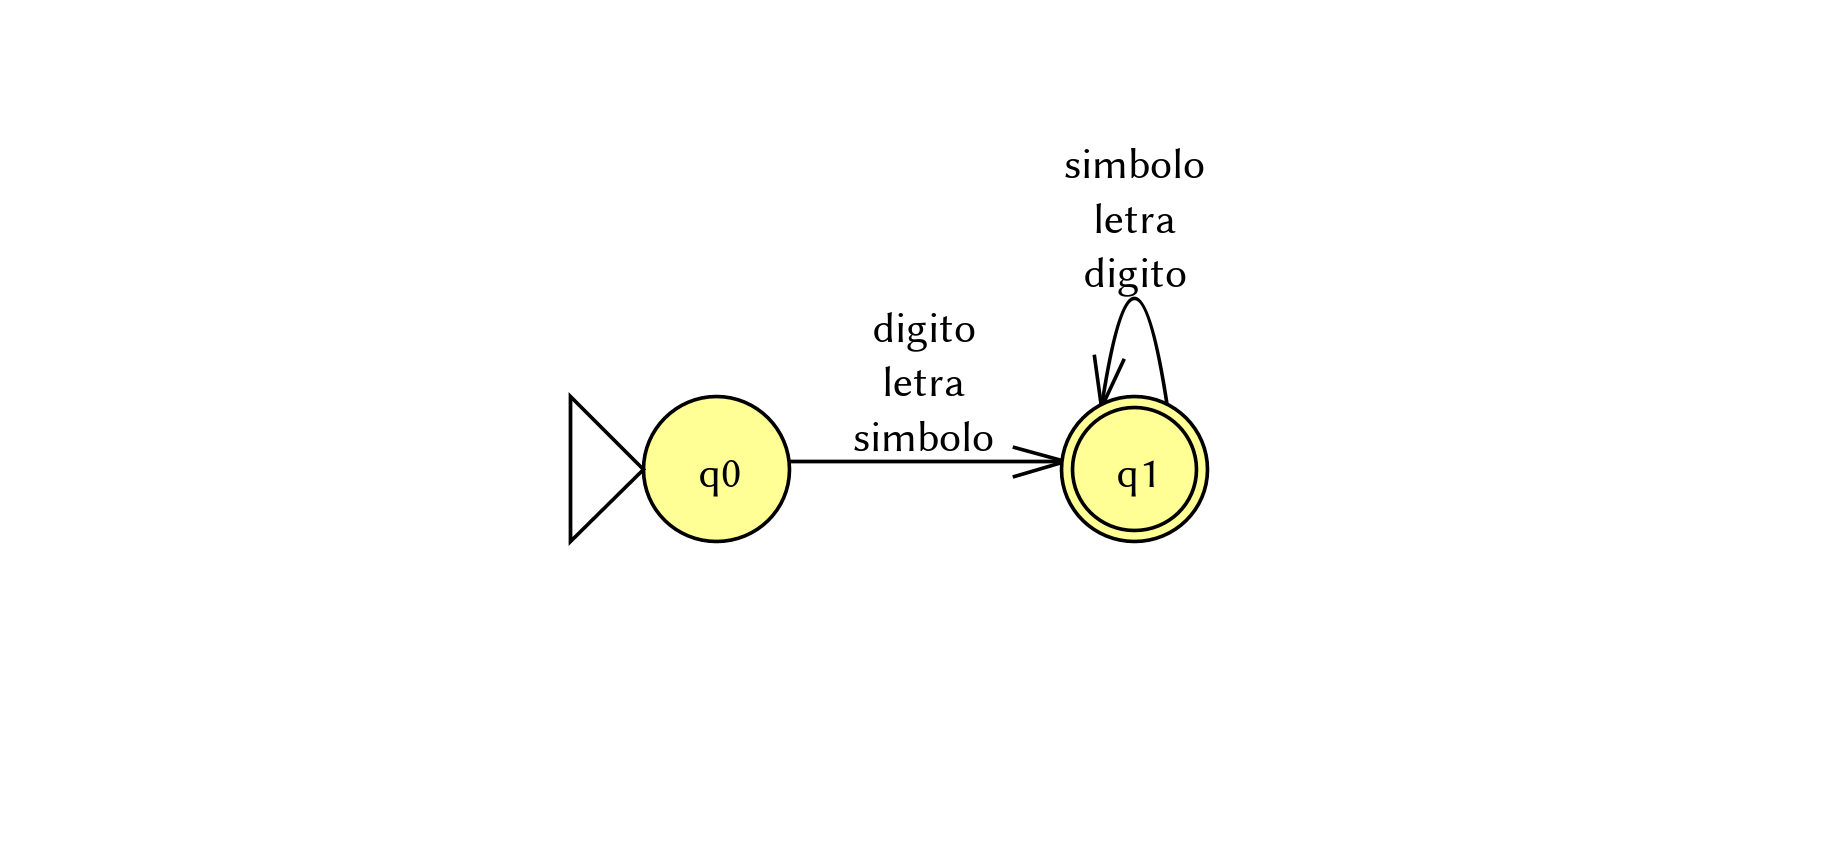
\includegraphics[width=.4\linewidth]{automatas_finitos/textoDrt.png}
	\caption{Automata finito para texto}
	\label{fig:texto}
\end{figure}

\subsection{nombre}
\label{sub:nombre}
Esta expresión se utiliza a lo largo del documento para hacer referencia a
cadenas de texto que identifiquen un elemento del lenguaje, como por ejemplo,
utilizando con la palabra \texttt{class} este pasaría a definir el nombre de la
clase, si se utiliza con en un contexto de atributo, este pasaría a formar
parte del nombre que identifica a ese atributo, a continuación se presenta la
gramática libre de contexto y la expresión regular para un elemento
\texttt{nombre} dentro del lenguaje:

Primero se realiza la definicion de una herrameinta que nos permita el uso
recursivo de \texttt{letra}, \texttt{simbolo} y \texttt{digito}. Si bien esto
se parece bastante a lo que se expone en la \texttt{Subsección \ref{sub:texto}}
per se tiene la necesidad de restringir el uso de símbolos a unicamente el uso
del guión bajo ``\_''.

\begin{lstlisting}[basicstyle=\footnotesize\ttfamily, caption={BNF intermedio
definición nombre}]
  <nombre-texto> ::= <letra|digito|"_"> <nombre-texto>
\end{lstlisting}

\begin{lstlisting}[basicstyle=\footnotesize\ttfamily, caption={BNF para un
nombre}]
  <nombre> ::= <letra> <nombre-texto>
\end{lstlisting}

En cuanto la expresión regular para la expresión anterior:

\begin{lstlisting}[basicstyle=\footnotesize\ttfamily, caption={regex para un
nombre}]
	Regex: /[a-zA-Z][a-zA-Z0-9]*/
\end{lstlisting}

\subsection{visibilidad}
\label{sub:visibilidad}
La visibilidad, como ya se explicó implicitamente en la descripción de algunas
de las palabras reservadas expuestas en la \texttt{Sección
\ref{sec:palabrasreservadas}}, tiene la función de establecer que miembros del
modelo tienen acceso ciertos elementos, el hecho de que estas esten compuestas
de palabras reservadas hace que su generalización con componentes de mas bajo
nivel descritos en las \texttt{Secciones \ref{sub:letra}},
\texttt{\ref{sub:digito}} y \texttt{\ref{sub:nombre}} no sea posible, por esta
razón se hace la descripción con los componentes literales que hacen a la
visibilidad.

La notacion BNF para la visibilidad es como se expone a continuación:

\begin{lstlisting}[basicstyle=\footnotesize\ttfamily]
  <visibilidad> ::= public | private | protected | derivate | package
\end{lstlisting}

Si bien esto permiten describir la visibilidad de los componentes del modelo,
según la especificación UML, en su totalidad, en el apartado
\ref{sec:simbolosespeciales} expone que el lenguaje preserva la naturaleza
gráfica de UML permitiendo que el usuario utilice simbolos para la definición
de visibilidad en diferentes componentes de un modelo, por lo tanto, teniendo
esto en consideración, la nueva expresión BNF para la \texttt{visibilidad} es
como sigue:

\begin{lstlisting}[language=Java, basicstyle=\footnotesize\ttfamily]
  <visibilidad> ::= public | + | private | - | protected | # |
	derivate | / | package | ~
\end{lstlisting}

También se presenta la expresion regular correspondiente a la notatión
presentada anteriormente:

\begin{lstlisting}[language=Java, basicstyle=\footnotesize\ttfamily]
	Regex: /(public|+|private|-|protected|#|derivate|/|package|~)/
\end{lstlisting}

\subsection{tipo}
\label{sub:tipo}
Este componente permite identificar la naturaleza de metodos y atributos dentro
de un modelo, estos, al igual que los componentes de la \texttt{visibilidad}
explicados en la \texttt{Subsección \ref{sub:visibilidad}}, están basados en
literales que forman parte del conjunto de palabras reservadas del lenguaje,
esta es la razon por la cual el \texttt{tipo} tampoco se puede generalizar como
también es mencionado en la subsección anterior.

El tipo se puede describir de la siguiente manera:

\begin{lstlisting}[basicstyle=\footnotesize\ttfamily]
	<tipo> ::= integer | double | float | long | boolean |
	string | char | list<<tipo>> | set<<tipo>>
\end{lstlisting}

en cuanto a la expresión regular que concierne a la gramática anterior se
describe a continuación como:

\begin{lstlisting}[basicstyle=\footnotesize\ttfamily]
	Regex: //
\end{lstlisting}

